\documentclass[a4paper,dvips,12pt,oneside,onecolumn,final,openright]{book}

\title{\textbf{Face De-identification with Preserving Expressions in Different Poses}}
\author{\textbf{Song Yuhao}}
\date{September 2015}


%%----------------------------------------------------------------------------%%
%%    Packages to include                                                     %%
%%----------------------------------------------------------------------------%%


% for general layout
%\usepackage{times}
%\usepackage{thesisStyle}
\usepackage{calc}
\usepackage{tocbibind}
\usepackage{indentfirst}
\usepackage{fancyhdr}
\usepackage{setspace}
\usepackage{titlesec}
\usepackage[font=footnotesize, labelfont={bf}, margin=1cm]{caption}
% for tables
\usepackage{array}
\usepackage{dcolumn}
\usepackage{multirow}
\usepackage{tabularx}
\usepackage{picinpar}
\usepackage{longtable}
% for maths
\usepackage{amsmath}
\usepackage{amssymb}
\usepackage{theorem}
\usepackage{bm}
% for SI symbols
%\usepackage[thinspace,amssymb]{SIunits}

% for graphics
\usepackage{color}
\usepackage{graphicx}
\DeclareGraphicsExtensions{.eps,.pdf,.jpg,.png}
\DeclareGraphicsRule{.png}{eps}{.bb}{}
%\usepackage[tight,FIGBOTCAP,TABBOTCAP,hang]{subfigure}
\usepackage[footnotesize]{subfigure}
\usepackage{rotating}


% for algorithms
%\usepackage[plain,section]{algorithm}
\usepackage{algorithm}
\usepackage{algorithmic}
\usepackage{ifthen}
%%----------------------------------------------------------------------------%%
%%    Page layout                                                             %%
%%----------------------------------------------------------------------------%%
\renewcommand{\cleardoublepage}{\clearpage}
%% from setspace.sty: 1.5 spacing for 11pt font
\renewcommand{\baselinestretch}{1.5}

%% from vmargin.sty
\setlength{\hoffset}{-1in} \setlength{\voffset}{-1in}
\setlength{\footskip}{2.5cm} \setlength{\headsep}{1.5cm}
\setlength{\topmargin}{1cm}
\setlength{\headheight}{2\baselineskip}
\setlength{\oddsidemargin}{3.5cm}
\setlength{\evensidemargin}{3.5cm}
\setlength{\textwidth}{\paperwidth-\oddsidemargin-\evensidemargin}
\setlength{\textheight}{\paperheight-\topmargin-\headheight-\headsep-\footskip-1in}
\setlength{\parskip}{1.5ex} \setlength{\parindent}{2em}
\setlength{\partopsep}{5pt}

% the right margin of TOC, except the line with page number
\makeatletter
\renewcommand{\@tocrmarg}{.5in}
\makeatother

% subfigure and subtable are listed in TOC also
\setcounter{lofdepth}{2}\setcounter{lofdepth}{2}
\setcounter{tocdepth}{3} \setcounter{secnumdepth}{3}


% from subfigure.sty: just to make the label field wider
\makeatletter
\renewcommand{\l@subfigure}{%
  \@dottedxxxline{\ext@subfigure}{2}{3.9em}{3.1em}}
\renewcommand{\l@subtable}{%
  \@dottedxxxline{\ext@subtable}{2}{3.9em}{3.1em}}
\makeatother

% new math operator for CI3/5/7
\DeclareMathOperator*{\sgn}{sgn}


%%----------------------------------------------------------------------------%%
%%    Various environments                                                    %%
%%----------------------------------------------------------------------------%%

\theoremstyle{break} \theorembodyfont{\normalfont}
\newtheorem{definition}{Definition}[section]
\newtheorem{theorem}{Theorem}[section]

\newcommand{\QED}{%
  \ifmmode % if math mode, assume display: omit penalty etc.
  \else \leavevmode\unskip\penalty9999 \hbox{}\nobreak\hfill
  \fi
  \quad\mbox{\rule[0pt]{1.5ex}{1.5ex}}}
\newcommand{\disableQED}{\renewcommand{\QED}{}}
\newenvironment{proof}%
  {\setlength{\parindent}{0pt}\textbf{Proof: }}%
  {\QED}

\newcounter{cases}
\newenvironment{Cases}%
  {\begin{list}%
    {Case \arabic{cases}:}%
    {%
      \usecounter{cases}%
      \setlength{\labelsep}{5pt}%
      \settowidth{\labelwidth}{Case }
      \setlength{\leftmargin}{\labelwidth}
      \advance\labelwidth 20pt
      \advance\leftmargin 25pt
      \setlength{\listparindent}{0pt}%
      \setlength{\itemindent}{0pt}%
    }%
  }%
  {\end{list}}


%%----------------------------------------------------------------------------%%
%%    Environment for Title Page                                              %%
%%----------------------------------------------------------------------------%%

\makeatletter
\renewcommand{\maketitle}
{%
  \begin{titlepage}
    %\renewcommand{\baselinestretch}{1}%
    \begin{center}
      {\LARGE\@title\par}
      \vspace*{\stretch{5}}
      {\Large\@author\par}
      \vspace*{\stretch{5}}
      \textbf{
        A thesis submitted in partial fulfilment of the requirements\\
        for the degree of\\
        Master of Philosophy\\}
      \vspace*{\stretch{5}}
      \begin{table}[!h]
      \centering
      \begin{tabular}{r@{\textbf{: }}l}
        \textbf{Principal Supervisor}& \textbf{Prof. YUEN Pong Chi}\\
        \textbf{Co-Supervisor}& \textbf{Dr. ZHANG Hui}\\
      \end{tabular}
      \end{table}
      \textbf{Hong Kong Baptist University\\}
      {\large\textbf{\@date}\par}
    \end{center}
  \end{titlepage}
} \makeatother

%%----------------------------------------------------------------------------%%
%%    Environment for Declaration                                             %%
%%----------------------------------------------------------------------------%%

\makeatletter
\newcommand{\makedeclaration}
{
\begin{center}\textbf{DECLARATION}\end{center}
\addcontentsline{toc}{chapter}{Declaration}

I hereby declare that this thesis represents my own work which has
been done after registration for the degree of MPhil at Hong Kong
Baptist University, and has not been previously included in a thesis
or dissertation submitted to this or any other institution for a degree,
diploma or other qualifications.
\vspace*{2.5cm}
\begin{flushright}
\begin{tabular}{r@{: }l@{}}
Signature& \underline{\hbox to 30mm{}} \\
Date&\@date\\
\end{tabular}
\end{flushright}
%\pagestyle{plain}%
} \makeatother

%%----------------------------------------------------------------------------%%
%%    Environment for Abstract                                                %%
%%----------------------------------------------------------------------------%%

\makeatletter
\newenvironment{abstract}%
{
\if@twocolumn
    \@restonecoltrue\onecolumn
  \else
    \@restonecolfalse\newpage
  \fi
  \begin{table}
  \begin{center}
  \begin{tabular*}{1\textwidth}{ @{\extracolsep{\fill}} lr }
  SONG Yuhao& Master of Philosophy\\
  Hong Kong Baptist University&\@date\\
  \end{tabular*}
  \end{center}
  \end{table}
  \begin{center}
  \large
  \@title\\
  \vspace*{1.5cm}
  \textbf{Abstract}
  \vspace*{2.5cm}
  \end{center}
%Start Abstract
\addcontentsline{toc}{chapter}{Abstract}
%%%%%%%%%%%%%%%%%%%%%%%%%%%%%%%%%%%%%%%%%%%%%%%%%%%%%%%%%%%%%%%%%%%%%%%%%%%%%%%
%   Abstracts                                                                 %
%%%%%%%%%%%%%%%%%%%%%%%%%%%%%%%%%%%%%%%%%%%%%%%%%%%%%%%%%%%%%%%%%%%%%%%%%%%%%%%
%\pagenumbering{roman} \setcounter{page}{1}
%\chapter*{}
%\chapter*{Abstract\markboth{Abstract}{Abstract}}
%Mark 'Abstract' both even and odd markers

}%
\makeatother

%%----------------------------------------------------------------------------%%
%%    Environment for Acknowledgements                                             %%
%%----------------------------------------------------------------------------%%

\makeatletter
\newcommand{\makeAck}
{
\chapter*{Acknowledgements}
\addcontentsline{toc}{chapter}{Acknowledgements}
%%%%%%%%%%%%%%%%%%%%%%%%%%%%%%%%%%%%%%%%%%%%%%%%%%%%%%%%%%%%%%%%%%%%%%%%%%%%%%%
%   Acknowledgements                                                          %
%%%%%%%%%%%%%%%%%%%%%%%%%%%%%%%%%%%%%%%%%%%%%%%%%%%%%%%%%%%%%%%%%%%%%%%%%%%%%%%
%\chapter*{Acknowledgements\markboth{Acknowledgements}{Acknowledgements}}

This project would not have been completed without the support of many people. I highly appreciate my supervisor, Hui Zhang, who enlightened me from knowing nothing in this field and helped me make sense of my confusion. Thanks to my principle supervisor, Pong-Chi Yuen, who offered guidance and support during the period of study. Thanks to Hong Kong Baptist University for providing me a monthly studentship for my study. And finally, thanks to my parents and numerous friends who always offering support and love.



} \makeatother
%%----------------------------------------------------------------------------%%
%%    Environment for Notation                                                %%
%%----------------------------------------------------------------------------%%

\makeatletter
\newcommand{\makenotation}
{
\chapter*{Notation}
\addcontentsline{toc}{chapter}{Notation}
\section*{Camera Parameters}
\begin{table}[!h]
\begin{flushleft}
    \begin{tabular}{ c l }
    $f$ & Focal length\\
    ($u_0,v_0$)& Principal point \\
    \end{tabular}
\end{flushleft}
\end{table}
\section*{Operators}
\begin{table}[!h]
\begin{flushleft}
    \begin{tabular}{ c l }
    $a\times b$ & Cross product of vectors $a$ and $b$\\
    $\textbf{M}^\textbf{T}$ & Transpose of matrix $M$\\
    $\textbf{M}^{-1}$ & Inverse of matrix $M$\\
    $\mp$ & Minus or plus\\
    \end{tabular}
\end{flushleft}
\end{table}
\section*{Named Variables}
\begin{flushleft}
    \begin{longtable}{ c l }
    $\textbf{e}$ & epipole\\
    $\overline{\textbf{a}}$ & Hypothesis of $a$\\
    $\omega$ & Imaged absolute conic\\
    \textbf{K} & Calibration matrix\\
    \textbf{P} & Projection matrix\\
    \textbf{R} & Camera orientation\\
    $\textbf{R}_y$ & Rotation matrix respects to rotation axis\\
    $\textbf{T}$ & Translation vector\\
    $M$ & Mirror\\
    $C$ & Camera\\
    $\Pi$ & The rotation plane\\
    $\textbf{l}_h$ & The horizon line or vanishing line of $\Pi$\\
    $\textbf{m}$ & The point that mirror plane intersects with $\textbf{l}_h$\\
    $\textbf{v}$ & Vanishing point \\
    $\alpha$ & The angle between $C$ and $M_1$\\
    $\beta$ & The angle between $C$ and $M_2$\\
    $\theta$ & The angle between two mirrors\\
    $\textbf{l}_s$ & The imaged rotation axis and the vanishing line of Y-axis\\
    $\textbf{v}_z$ & The vanishing point of Z-axis\\
    $\textbf{v}_x$ & The vanishing point of X-axis\\
    $\textbf{v}_y$ & The vanishing point of Y-axis\\
    \{a,b;c,d\} & Cross ratio of vector $a$, $b$, $c$, $d$\\
    \end{longtable}
\end{flushleft}
%\pagestyle{fancy} \fancyhf{}
%\fancyhead[LO]{\slshape NOTATION}
%\fancyhead[RE]{\slshape NOTATION}
%\fancyfoot[C]{\it \thepage}
} \makeatother
%%----------------------------------------------------------------------------%%
%%    Environment for CV                                                      %%
%%----------------------------------------------------------------------------%%

\makeatletter
\newcommand{\makecv}
{
\if@twocolumn
    \@restonecoltrue\onecolumn
  \else
    \@restonecolfalse\newpage
  \fi
\begin{center}\textbf{CURRICULUM VITAE}\end{center}
\addcontentsline{toc}{chapter}{CURRICULUM VITAE}
Academic qualifications of the thesis author, SONG Yuhao:
\begin{itemize}
  \item Received  the degree of Bachelor of Science(Honours) from Beijing Normal University - Hong Kong Baptist University United International College (UIC), September 2009.
\end{itemize}
\vspace*{1cm}
\begin{flushright}
\@date
\end{flushright}
\pagestyle{plain}%
} \makeatother


%%----------------------------------------------------------------------------%%
%%   Various conventions                                                      %%
%%----------------------------------------------------------------------------%%

\newcommand{\NI}{\noindent}
\newcommand{\LL}{\ensuremath{\mathcal{L}}}
\newcommand{\RR}{\ensuremath{\mathcal{R}}}
\newcommand{\CC}{\ensuremath{\mathcal{C}}}
\newcommand{\DD}{\ensuremath{\mathcal{D}}}
\newcommand{\TT}{\ensuremath{\mathcal{T}}}
\newcommand{\EE}{\ensuremath{\mathcal{E}}}
\newcommand{\SSS}{\ensuremath{\mathcal{S}}}
\newcommand{\T}[1]{\ensuremath{\mathit{#1}}}
\newcommand{\N}[1]{\ensuremath{\overline{#1}}}
\newcommand{\Count}[2][]%
  {\ensuremath{\T{count}\ifx#1\undefined\else_{#1}\fi({#2})}}
\newcommand{\Support}[2][]%
  {\ensuremath{\T{supp}\ifx#1\undefined\else_{#1}\fi({#2})}}
\newcommand{\GrowthRate}[3]{\ensuremath{\T{growthRate}\ifx#2\undefined\else_%
  {\ifx#1\undefined\else{#1}\rightarrow\fi{#2}}\fi({#3})}}
\newcommand{\substr}{\sqsubset}
\newcommand{\substreq}{\sqsubseteq}
\newcommand{\prefix}{\prec}
\newcommand{\suffix}{\succ}
\newcommand{\emptystr}{\ensuremath{\varepsilon}}

\newcommand{\FUNCNAME}[1]{\item[{#1}]}
\newcommand{\INPUT}{\item[\textbf{Input:}]}
\newcommand{\INPUTT}{\item[\phantom{\textbf{Input:}}]}
\newcommand{\OUTPUT}{\item[\textbf{Output:}]}
\newcommand{\REMARK}{\item[\textbf{Remark:}]}
\newcommand{\REMARKK}{\item[\phantom{\textbf{Remark:}}]}
%\newcommand{\RETURN}{\textbf{return} }
%\newcommand{\STATEE}{\item[]}
\newcommand{\divider}{\par\mbox{}\hrule\mbox{}\par}

\newcommand{\PreserveBackslash}[1]{\let\temp=\\#1\let\\=\temp}
\let\PBS=\PreserveBackslash
\newcommand{\up}[1]{\raisebox{1.5ex}[0pt][0pt]{#1}}
\newcommand{\md}[1]{\multicolumn{2}{c|}{#1}}
\newcommand{\thickerspace}{\thickspace \thickspace}
\newcommand{\blob}{\rule[.2ex]{1ex}{1ex}}

\hyphenation{ac-know-ledge-ment} \hyphenation{data-bases}
\hyphenation{emer-ging} \hyphenation{sub-string}
\hyphenation{sub-strings} \hyphenation{se-quence}
\hyphenation{se-quences} \hyphenation{classi-fier}
\hyphenation{classi-fiers} \hyphenation{classi-fi-ca-tion}
\hyphenation{infre-quent} \hyphenation{research}
\hyphenation{threshold}


%%----------------------------------------------------------------------------%%
%%    Other stuff                                                             %%
%%----------------------------------------------------------------------------%%

\makeatletter
  \renewcommand{\@subcaption}[2]{%
    \begingroup
      \let\label\@gobble
      \def\protect{\string\string\string}%
      \xdef\@subfigcaptionlist{%
        \@subfigcaptionlist,%
        {\numberline {\@currentlabel}%
      \noexpand{\ignorespaces #2}}}%
    \endgroup
  \@nameuse{@make#1caption}{\@nameuse{@the#1}}}
\makeatother


%%----------------------------------------------------------------------------%%
%%    Content of thesis                                                       %%
%%----------------------------------------------------------------------------%%

%%---------------------%%
\begin{document}
%\setboolean{@twoside}{true}
%%---------------------%%
\maketitle
\frontmatter
\pagestyle{fancy} \fancyhf{} %\fancyhead[LE,RO]{\it \thepage}
%\fancyhead[LO]{\slshape \rightmark}
%\fancyhead[RE]{\slshape \leftmark}
\fancyfoot[C]{\it \thepage}
\renewcommand{\headrulewidth}{0pt}
\renewcommand{\footrulewidth}{0pt}
\fancypagestyle{plain}%
{
  \fancyhf{}
  \fancyfoot[C]{\it \thepage}
  \renewcommand{\headrulewidth}{0pt}
  \renewcommand{\footrulewidth}{0pt}
}

\makedeclaration
\begin{abstract}
%%%%%%%%%%%%%%%%%%%%%%%%%%%%%%%%%%%%%%%%%%%%%%%%%%%%%%%%%%%%%%%%%%%%%%%%%%%%%%%%
%   Abstracts                                                                 %
%%%%%%%%%%%%%%%%%%%%%%%%%%%%%%%%%%%%%%%%%%%%%%%%%%%%%%%%%%%%%%%%%%%%%%%%%%%%%%%
%\pagenumbering{roman} \setcounter{page}{1}
%\chapter*{}
%\chapter*{Abstract\markboth{Abstract}{Abstract}}
%Mark 'Abstract' both even and odd markers

\end{abstract}
\makeAck
%%---------------------%%

%%---------------------%%
\tableofcontents \listoftables \listoffigures
\makenotation
%%---------------------%%
\mainmatter
%%---------------------%%
\pagestyle{fancy} \fancyhf{} %\fancyhead[LE,RO]{\thepage}
%\fancyhead[LO]{\slshape \rightmark}
%\fancyhead[RE]{\slshape \leftmark}
\fancyfoot[C]{\thepage}
\renewcommand{\headrulewidth}{0pt}
\renewcommand{\footrulewidth}{0pt}
\fancypagestyle{plain}%
{
  \fancyhf{}
  \fancyfoot[C]{\thepage}
  \renewcommand{\headrulewidth}{0pt}
  \renewcommand{\footrulewidth}{0pt}
}

%%%%%%%%%%%%%%%%%%%%%%%%%%%%%%%%%%%%%%%%%%%%%%%%%%%%%%%%%%%%%%%%%%%
%                                                                 %
%                            CHAPTER ONE                          %
%                                                                 %
%%%%%%%%%%%%%%%%%%%%%%%%%%%%%%%%%%%%%%%%%%%%%%%%%%%%%%%%%%%%%%%%%%%

\chapter{Introduction}

\section{Background}

The problem that keeps balance between privacy protection and expression preservation is addressed in this paper. 
Face de-identification 

\par
Active appearance model (AAM) have been successfully applied to model the space of human face for decades. The AAM could be used in both face recognition and facial expression recognition methods. What is the difference role in the two recognition methods?(2015-5-11)

\par
The practical situations are eager to find a way to protect human identity privacy. Mosaic and blur.

% Social experiment example
\par
Imaging a situation in a social experiment, the researchers wish to observe volunteers' direct reactions to some events. As an important channel in communication, facial expression is not tolarable to be ignored for it is the most direct reflection of a person's emotional state. In general, the results of these social experiment are recorded by images or videos. 


% Hospital surveillance example
\par
Hospital surveillance videos are expected to contain rich health information including clinical reactions, effects after some treatments which are anaylzed from behaviors or expressions of the patients. Among the information, the identities of patients are so sensitive that it is forbidden to share the surveillance video with other researchers. For this reason, an technique that could protect patients' identity privacy and preserve most useful expression and behavior information simultanously are eager to be found thus making it possible to share the useful surveillance materials without leaking patients' identity information.

% Television example
\par
A common privacy protection measure is applying mosaic in interviewee's face region in television interview. 
However, the mosaic hide both identity and expression information storing in face, lefting the only way for audience to understand content by listening the sound. Mehrabian illustrates that the spoken words of a message contributes only for $7\%$ to the effect of the message as a whole, the voice intonation contributes for $38\%$, while the facial expression of the speaker contributes for $55\%$ to the effect of the spoken message ~\cite{Meh68}. Illustrated as the data above, facial expressions overcomes spoken words obviously in communication. Therefore, it is necessary to invent a new technique that is able to protect face identity information and preserve the facial expressions simultanously. 

% Ross example, the importance of expressions
\par
To show how important the expressions are in communication, four frames from a movie are taken. In the top right frame of Figure \ref{expression}, the person called Ross says "my best friend and my sister" with an angry expression after realizing that his sister and best friend are in a relationship with him unknown. After the explanation of top left frame and bottom right frame, he knows his sister and his best friend fell in love with each other and are both serious to the relationship, so he becomes supportive to the lovers. In the bottom left frame, Ross says the same words, "my best friend and my sister", with a happy expression. Even the voice and intonation are not available and the spoken words are totaly the same, the meanings shown from the figures are obviously opposite analyzed from the expressions. 
\begin{figure}
  \centering
  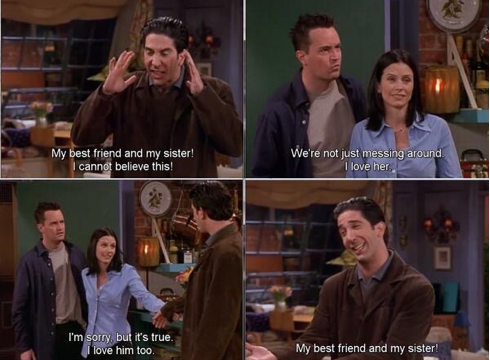
\includegraphics[width=0.9\textwidth]{figure/sisFri.png} 
  \caption{An example of communication with different expressions}
  \label{expression}
\end{figure}

% how to evaluate expression
Facial Action Coding System (FACS), developed by a Swedish anatomist named Carl-Herman Hjortsjö, is a system that classify the human facial movement by the appearance of the face ~\cite{facs70}. 


% The importance of privacy
\par
Door lock system through face recognition is a rapidly developed technology in security area. A potential vulnerable attacking method is reconstructing a 3D human face model through a video sequence which is definitely easy to get and then use the 3D printer to get a real face object which could be used to cheat the door lock system. 

Face recognition ATM



% pose
Pose estimation of faces are usually addressed assuming the face detection problem has been solved. 3D models and 2D view-based models are usually used. 


The essential of face de-identification problem is a face reconstruction process deleting the identity specific factors in the face.  
The key is how to build the database and train. 

The result of our project would be a synthetic face that would not be recognized by automatic face recognition algorithm but would be figured out by expression recognition algorithm. We are going to build a model with three kinds of parameters: identity, pose, expressions. 

A question: the appearance of a face. The result would be nobody, but it looks natural like the normal people. Why would it looks like a normal person?

Make it clear what data utility is. 

The problem is difficult as the appearance of a face could vary greatly due to the environmental factors like illumination and image noise or resolution. 

\section{Objectives}
We wish to create a new face model in which all identity factors are extracted independently and then reconstruct the face image with the de-identified identity facotrs. 

definition of identity privacy and data utility

% Contribution
\section{Contributions}
\par


% Structure of the whole thesis
\section{Outline of this thesis}
\par 
The rest of this thesis is arranged as follows. 
\chapter{Related Work}

\section{Ad-hoc methods}
	Simple distortion methods are applied to the image privacy protection field such as pixelation and blurring. The pixelation method subsamples the image and the blurring method smoothes images with some filters like Gaussian filter or average filter ~\cite{Agrawal09,Boyle00}. Both by destorying the original image information, pixelation and blurring make a trade between privacy information and image quality. Although these two methods are widely used in practical situations like TV interviews, they suffer from the same risk proposed in ~\cite{Newton05} called parrot attack. General face recognition algorithms figure out the identity by computing the similarity between the target image and database images. Blur and pixelation destory the target image information so that the target image is not similar to any image in database. Parrot attack would preprocess all the database images with pixelation or blurring, then applies face recognition algorithms to pixelated or blurred images so that target images and database images are preprocessed with the similar procedures. 

	\par
	Two more de-identificaiton methods are introduced in ~\cite{Winkler14}: blanking and encryption. The intuitive blanking method in face de-identificaiton is to cut the face region off and replace the region with black color. It also could be extended to paint the region of interest, like face, with background images  ~\cite{inpaint09,Qureshi09}. Compared with other de-identification methods introduced before, encryption has the advantage in recovery ~\cite{Boult05}. With a proper key, the encrypted image is always available to be decrypted so that the image remains useful even if it is covered by a snowboard. These two methods cover image information including both identity and facial expressions. It is the balance between privacy and data utilization that should be the key point in face de-identification. Protecting the identity privacy while preserving facial expressions simultanously is the purpose of our research. 
	
	\par
	Dufaux ~\cite{dufaux08} introduced a privacy protection method using in video sequence by scrambling the locations of pixels in a rectangle range. By controling the range size, different degrees of fuzzy results could be produced. 

	The images comes from ~\cite{dufaux08}.
	% whether place four images here
	\begin{figure}[!htb]
		  \centering
		  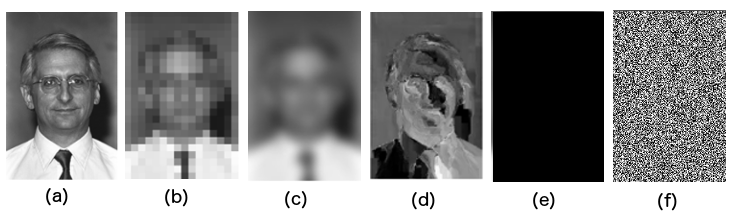
\includegraphics[width=0.9\textwidth]{figure/adhoc.png} 
		  \caption{(a) the origianl image; (b) Pixelation; (c) blurring; (d) scrambling; (e) blanking; (f) encryption}
		  \label{expression}
	\end{figure}


\section{K-anonymity based methods}

	General solutions model face shape and appearance separately. 
\chapter{Proposed Methodology}

Procrustes analysis, named after a bandit from Greek mythology who streches or cut off his victim to his bed, is used to analyse the distribution of a set of shapes. Shape is all geometrical information that remains when location, scale and rotational effects are filtered out from an object ~\cite{IMM2002-0403}. 

For ASM (Active Shape Model), the training data set contains arbitrary size images for the Procrustes analysis would normalize the data.

Diagram 
\chapter{Experiment and Results}

he proposed face de-identification approach has been implemented. Recently, I spend most time in setting up experiments and the corresponding analysis. This report would display the de-identified face images in both shape and appearance level. To inspect the ability of protecting privacy, face recognition algorithm is applied to the original face images and de-identified results. On the other hand, expression recognition algorithm is used to check whether the approaches are able to preserve the useful information.  


\section{De-identified results}
In our experiment, CMU PIE face database is firstly used to test the proposed approaches. Images from 20 subjects are chosen to build the tensor model. Each one of them has 3 poses: frontal, left profile, right profile, and 2 expressions: normal and smile. Other images are for testing. The program is executed in Matlab. The Sandia tensor toolbox is used to analyze the tensor. To show the flexibility of our proposed framework, another face database, IMM, is also tested. The types of pose and expression involved in IMM are the same as CMU PIE, but there are no smile images for right profile and left profile poses. Therefore, expression dimension is not included in IMM experiment. 

A face image is processed in two levels: shape and appearance. Similar with AAM, the feature points in one face compose its shape. Different faces in different poses yield a unique shape. The de-identified algorithms could transform a shape into a different one that represents a similar pose. Appearances are the pixels in an image. The de-identified appearance is expected to be different and normal. In plain words, the result face is normal looking. No distortion or other unnatural appearance would show. The most important is people could not recognize the person identity in results based on original images.


	\subsection{Proposed approach}

	All the group images appear in this report is arranged as: the right is the original image and the left is de-identified result. Fig.\ref{fig:shape_recon} is a sample of shape de-identification. The shape data has been decomposed into multiple dimensions and we only modify the identity one, so the result is not the same with original shape but is in similar pose.

	\begin{figure}[!htb]
		  \centering
		  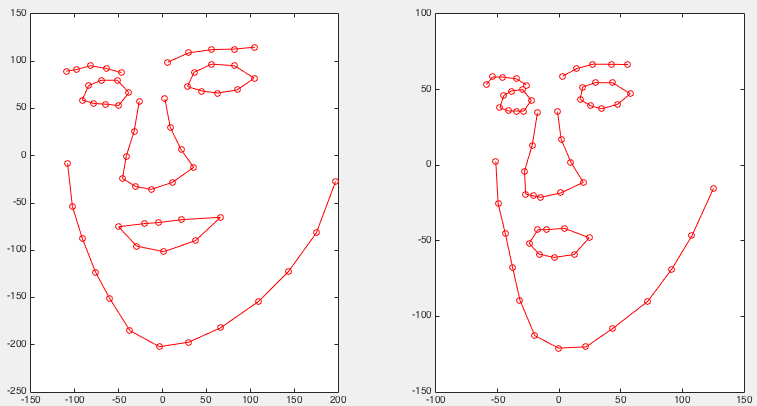
\includegraphics[width=0.6\textwidth]{figure/shape_recon}
		  \caption{Shape de-identification by proposed approach}
		  \label{fig:shape_recon}
	\end{figure}

	For the face shapes are not in the same size, all appearances are warped to a mean shape so that it is possible to compare different images. Therefore, the de-identified appearance should warp back to de-identified shape. That is the final result of our approach. Fig. \ref{fig:tensor_result_1} is one example of final result.

		\begin{figure}[!htb]
		  \centering
		  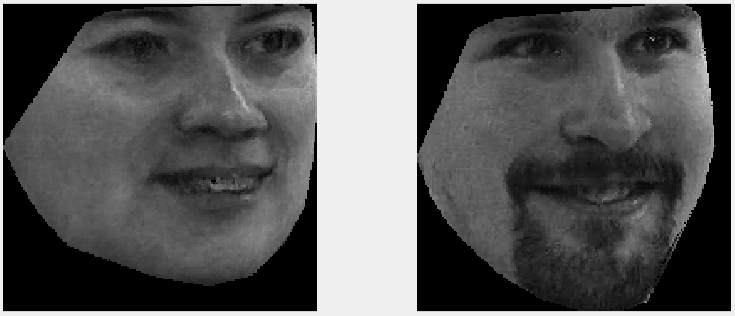
\includegraphics[width=0.6\textwidth]{figure/right_smile}
		  \caption{De-identified appearance warp back to de-identified shape}
		  \label{fig:tensor_result_1}
		\end{figure}

	The criteria of judgeing the result are:
	\begin{enumerate}
		\item the de-identified face is not the same one with the original face,
		\item the de-identified face is normal, containing no unnatural appearance like distortion.
	\end{enumerate}


	\subsection{k-same-M}
	K-same-M is one of the best face de-identification algorithms. It describes a face image by parameters of a model like AAM and then take the average of $k$ image parameters as a new one. At last, a new face image is reconstructed by the new parameters and the model. Since all parameters are in the same dimension, the result might lose more useful information than identity. Fig. \ref{fig:shape_k_s} is an example of shape de-identification. The original left profile pose is tranformed into frontal face. 

	\begin{figure}[!htb]
	  \centering
	  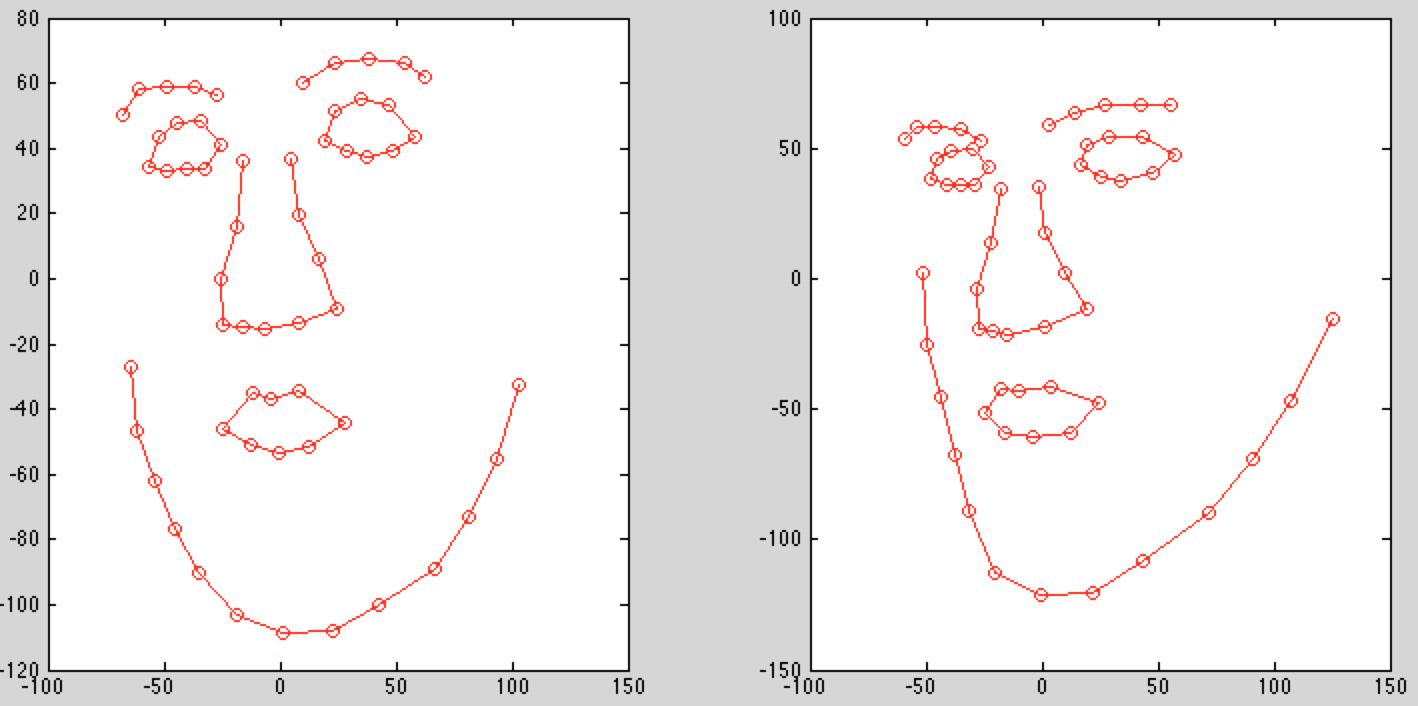
\includegraphics[width=0.6\textwidth]{figure/model_shape_1}
	  \caption{shape de-identification by k-same-M}
	  \label{fig:shape_k_s}
	\end{figure}

	De-identified appearance that warps back to de-identified shape forms the final result. If the face shape has been tranformed into a wrong one, the final result must be distorted and unnatural. Fig. \ref{fig:MkS} is an example of model-based de-identification results. The result has an obvious distortion in the face. 

	\begin{figure}[!htb]
	  \centering
	  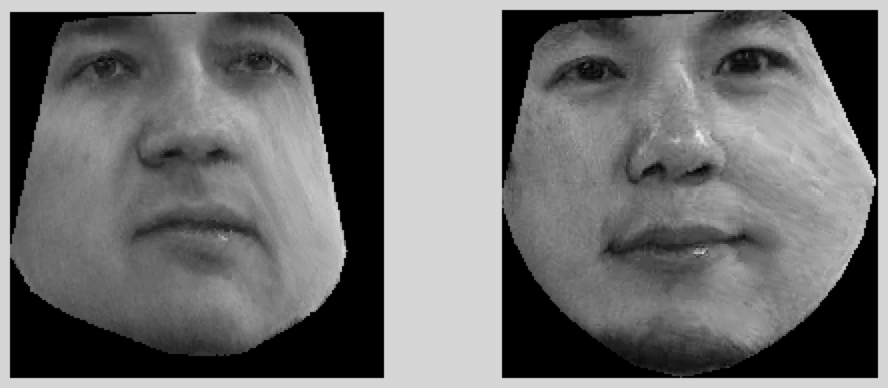
\includegraphics[width=0.6\textwidth]{figure/model_result}
	  \caption{de-identification by k-same-M}
	  \label{fig:MkS}
	\end{figure}

	K-same-M can definitely produce good results like Fig.\ref{fig:model_result}. However, the data utility of de-identified results can not be guaranteed. 

		\begin{figure}[!htb]
		  \centering
		  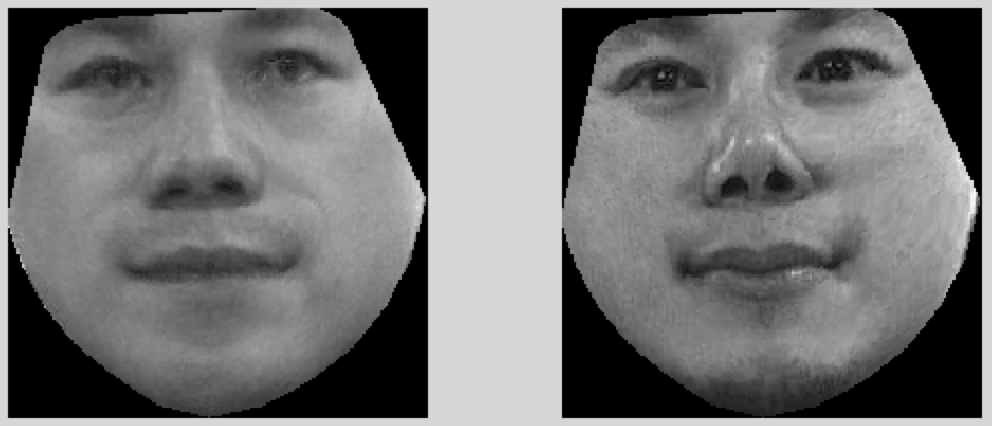
\includegraphics[width=0.6\textwidth]{figure/good_MkS}
		  \caption{model k same}
		  \label{fig:model_result}
		\end{figure}

\section{Recognition}

We have compared the proposed approach and existing ones in human vision level. The key point in face de-identification is to keep the ballance between privary protection and data utility preservation. We have addressed the expression is the most importatn information.This section would examine privacy and expression preservation in quantity.
	
	
	\begin{figure}[!htb]
	  \centering
	  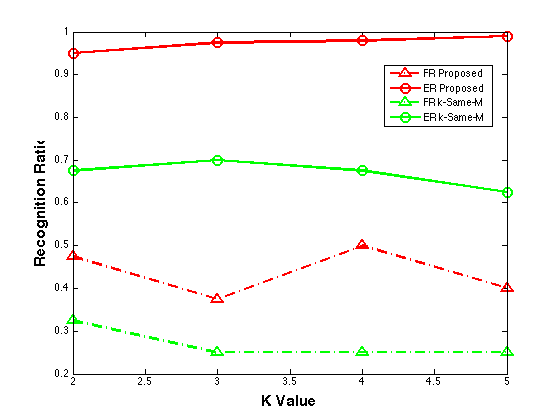
\includegraphics[width=0.8\textwidth]{figure/plotPic}
	  \caption{Recognition ratio.}
	  \label{fig:plotPic}
	\end{figure}

	Only frontal face images are used because the recognition algorithms performs best in these images. The PCA+KNN is chosen as the inspection method for face recognition (FR) and expression recognition (ER). This is the most stable recognition framework. Furthermore, it is easy to implement and performs well in small dataset. I think the inpsection method is not the key point of this experiment. It is the comparisons that really matter. 

	From the Fig. \ref{fig:plotPic}, we can see FR ratio of proposed approach is higher than k-same-M, but it is still acceptable. The ER ratio of proposed approach is increased to a high level. It is a trade-off between privacy and data utility. Our target is to preserve the data utility as large as possible when the privacy is protected well. 



The above is the objective testing. Further work about subjective testing is being prepared. I would design some questionnares for a survey about FR of de-identified results. 

\chapter{Conclusion and Future Works}


%%%---------------------%%
%\appendix
%%%---------------------%%
%\include{thesisApd}
%

%%---------------------%%
%\backmatter
%%---------------------%%
\bibliographystyle{splncs03}
\bibliography{reference/refs}
\makecv
\pagestyle{empty}
%\begin{thebibliography}{999}
%\addcontentsline{toc}{chapter}{\numberline{}\bibname}
%\include{tqwangBib}
%\end{thebibliography}

%%---------------------%%
\end{document}
%%---------------------%%


%%----------------------------------------------------------------------------%%
%%    End of thesis                                                           %%
%%----------------------------------------------------------------------------%%
